\documentclass{beamer}
\usepackage{listings}
\lstset{
%language=C,
frame=single, 
breaklines=true,
columns=fullflexible
}
\graphicspath{{./Figures/}}
\usepackage{gensymb}
\usepackage{subcaption}
\usepackage{url}
\usepackage{tikz}
\usepackage{tkz-euclide} % loads  TikZ and tkz-base
%\usetkzobj{all}
\usetikzlibrary{calc,math}
\usepackage{float}
\usepackage{extarrows}
\newcommand\norm[1]{\left\lVert#1\right\rVert}
\providecommand{\pr}[1]{\ensuremath{\Pr\left(#1\right)}}
\newcommand{\myvec}[1]{\ensuremath{\begin{pmatrix}#1\end{pmatrix}}}
\renewcommand{\vec}[1]{\mathbf{#1}}
\usepackage[export]{adjustbox}
\usepackage[utf8]{inputenc}
\usepackage{amsmath}
\usetheme{Boadilla}

\title{Construction of Quadrilateral}
\author{Sujal - AI20BTECH11020}

\date{\today}
\begin{document}

\begin{frame}
\titlepage
\end{frame}
\begin{frame}
\frametitle{Problem}
\begin{block}{Constuction Q-2.7}
Construct a quadrilateral $MIST$ where $MI = 3.5, IS = 6.5, \angle M = 75 \degree , \angle I = 105 \degree$ and $ \angle S = 120 \degree$.
\end{block}
The given information can be expressed as
    \begin{align}
    &\angle M = 75\degree = \alpha \label{eq 1}
    \\
    &\angle I = 105\degree = \beta \label{eq 2}
    \\
    &\angle S = 120\degree = \gamma \label{eq 3}
    \\
    &\norm{\vec{M}-\vec{I}} = 3.5 = a \label{eq 4}
    \\
    &\norm{\vec{I}-\vec{S}} = 6.5 = b \label{eq 5}
    \end{align}
\end{frame}
\begin{frame}
Let,
\begin{align}
\vec{M}=\myvec{0\\0},\vec{I}=\myvec{a\\0}
\end{align}
and Angle between $ST$ and +x-axis is $\theta$
\begin{align}
\theta &= 360\degree - (\beta + \gamma)\\
       &= 360\degree - (105\degree + 120\degree)\\
       &= 135\degree \label{eq a}
\end{align}
and we have to find $\vec{S}$ and $\vec{T}$.
\end{frame}
\begin{frame}
\begin{lemma}
\begin{align}
&\vec{S} =\vec{I} + b\vec{X} \text{ where } \vec{X} = \myvec{\cos (180\degree -\angle I)\\\sin (180\degree -\angle I)} \label{eq b}\\
&\vec{T} = x\vec{Y} \text{ where } \vec{Y} = \myvec{\cos\alpha\\\sin \alpha}\text{ and } x \in R^{+} \label{eq c}\\
&\text{Also, } \vec{T} = y\vec{Z}+\vec{S} \text{ where } \vec{Z} =  \myvec{\cos\theta\\\sin\theta} \text{ and }y \in R^{+} \label{eq d}
\end{align}
\end{lemma}
\end{frame}
\begin{frame}
Thus, 
from  \eqref{eq 2} and \eqref{eq 5} in \eqref{eq b},
\begin{align}
\vec{S} &=\myvec{3.5\\0} + 6.5\myvec{\cos 75\degree \\\sin 75\degree }\label{eq e}
\\
&=\myvec{5.18\\6.28}
\end{align}
Thus, 
from \eqref{eq c},\eqref{eq d} and \eqref{eq e}, we get
\begin{align}
&x\vec{Y} = y\vec{Z}+\vec{S}\\
&\myvec{\cos\alpha & -\cos\theta \\ \sin\alpha & -\sin\theta} \myvec{x \\ y} = \myvec{5.18\\6.28}
\end{align}
\end{frame}
\begin{frame}
The corresponding augmented matrix is 
\begin{align}
		\myvec{
		\cos\alpha & -\cos\theta & \vrule & 5.18 \\
		\sin\alpha & -\sin\theta & \vrule & 6.28 \\
	}
\end{align}
Using \eqref{eq 1} and \eqref{eq a} we get
\begin{align}
		\myvec{
		0.26 & 0.71 & \vrule & 5.18 \\
		0.97 & -0.71 & \vrule & 6.28 \\
	}
\end{align}
\end{frame}
\begin{frame}
We use the Guass Jordan Elimination method as:

\begin{align}
	\myvec{
		0.26 & 0.71 & \vrule & 5.18 \\
		0.97 & -0.71 & \vrule & 6.28 \\
	}
	\\
	\xleftrightarrow[]{R_2 \rightarrow R_2 - \frac{0.97}{0.26}R_1}
	\myvec{
		0.26 & 0.71 & \vrule & 5.18 \\
		0 & -3.20 & \vrule & -13.05 \\
	}
	\\
	\xleftrightarrow[]{R_2\rightarrow -\frac{1}{3.20}R_2}
	\myvec{
		0.26 & 0.71 & \vrule & 5.18 \\
		0 & 1 & \vrule & 4.08 \\
	}
	\\
	\xleftrightarrow[]{R_1 \rightarrow R_1 - 0.71 R_2}
	\myvec{
		0.26 & 0 & \vrule & 2.28 \\
		0 & 1 & \vrule & 4.08 \\
	}
	\\
	\xleftrightarrow[]{R_1 \rightarrow \frac{1}{0.26}R_1}
	\myvec{
		1 & 0 & \vrule & 8.77 \\
		0 & 1 & \vrule & 4.08 \\
	}
\end{align}
\end{frame}
\begin{frame}
Therefore, the values of $x$ and $y$ are:
\begin{align}
	x = 8.77 \\
	y = 4.08
\end{align}
And, from \eqref{eq c}
\begin{align}
\vec{T} &= 8.77 \myvec{ 0.26 \\ 0.97 }\\
		&= \myvec{ 2.28 \\ 8.51	}
\end{align}
Thus,
\begin{align}
\vec{M}=\myvec{0\\0}, \vec{I}=\myvec{3.5\\0}, \vec{S}=\myvec{5.18\\6.28}, \vec{T}=\myvec{2.28 \\ 8.51}
\end{align}
and the quadrilateral $MIST$ is the plotted in Fig \ref{plt}.
\end{frame}
\begin{frame}
\begin{figure}[!h]
\centering
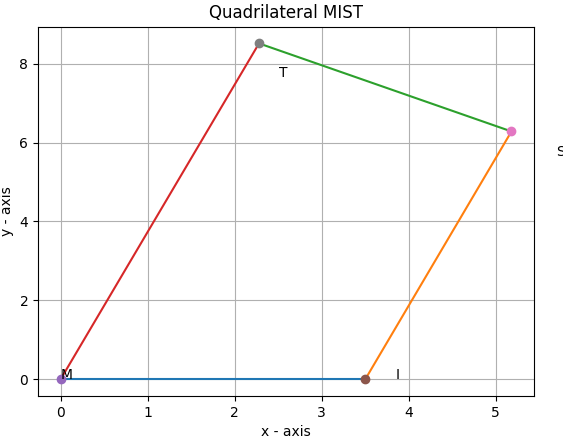
\includegraphics[ width=\columnwidth]{plot.png}
\caption{Quadrilateral MIST}
\label{plt}	
\end{figure}
\end{frame}
\end{document}